% Frank.Nielsen@acm.org

\documentclass[11pt]{article}
\usepackage{fullpage,amssymb,amsmath,hyperref,url}

\def\st{\ :\ }
\def\bbF{\mathbb{F}}
\def\eqdef{:=}
\def\eqnota{:=:}
\def\calY{\mathcal{Y}}
\def\dmu{\mathrm{d}\mu}
\def\dnu{\mathrm{d}\nu}
\def\calX{\mathcal{X}}
\def\calE{\mathcal{E}}
\def\bbR{\mathbb{R}}
\def\Var{\mathrm{Var}}
\def\KL{\mathrm{KL}}
\def\CS{\mathrm{CS}}
\def\calS{\mathcal{S}}
\def\dx{\mathrm{d}x}
\def\calE{\mathcal{E}}
\def\calD{\mathcal{D}}
\def\calX{\mathcal{X}}
\def\calF{\mathcal{F}}
\def\calP{\mathcal{P}}
\def\dmu{\mathrm{d}\mu}
\def\KL{\mathrm{KL}}
\def\JS{\mathrm{JS}}
\def\vJS{\mathrm{vJS}}
\def\IR{\mathrm{IR}}
\def\SME{\mathrm{SME}}
\def\MLE{\mathrm{MLE}}
\def\dtheta{\mathrm{d}\theta}
\def\Cauchy{\mathrm{Cauchy}}

\sloppy


\title{Distances, divergences, statistical divergences and diversities}
%\title{Distances and diversities}


\date{August 2021\\ (Last updated \today{})}

\author{Frank Nielsen\\ Sony Computer Science Laboratories Inc.\\ Tokyo, Japan}

\begin{document}
\maketitle

\vskip 0.5cm
This document is also available in PDF: \url{Distance.pdf} 
\vskip 0.5cm


This is a {\em working document} which will be (hopefully frequently) updated with materials concerning the discrepancies between two distributions/parameters or the diversities of a set of distributions/parameters.
There are many synonyms in the literature to measure the difference between two objects: 
Metrics, Distances, Discrepancies, deviations, deviances, dissimilarities, divergences, contrast functions or yokes (on product manifolds), etc.
Diversities generalize $2$-point distances by measuring the dispersion of a set of $n$ objects, usually using a centrality notion.

In mathematics, a distance is often considered to be a metric distance in a metric space which satisfies the following properties:

There is confusion in the literature where distance is also used as a synonym of a dissimilarity measure.

In information theory and statistics, we measure deviations between a probability measure and another probability measure using a statistical divergence.

In information geometry, a divergence is a smooth dissimilarity measure which shall satisfy the following conditions:

Divergences were formerly called contrast functions, a dualistic structure of information geometry can be built from a divergence.
 

\tableofcontents

%%%
\section{Jensen divergences and Bregman divergences}\label{sec:JDBD}
%%%%



\begin{figure}%
\centering
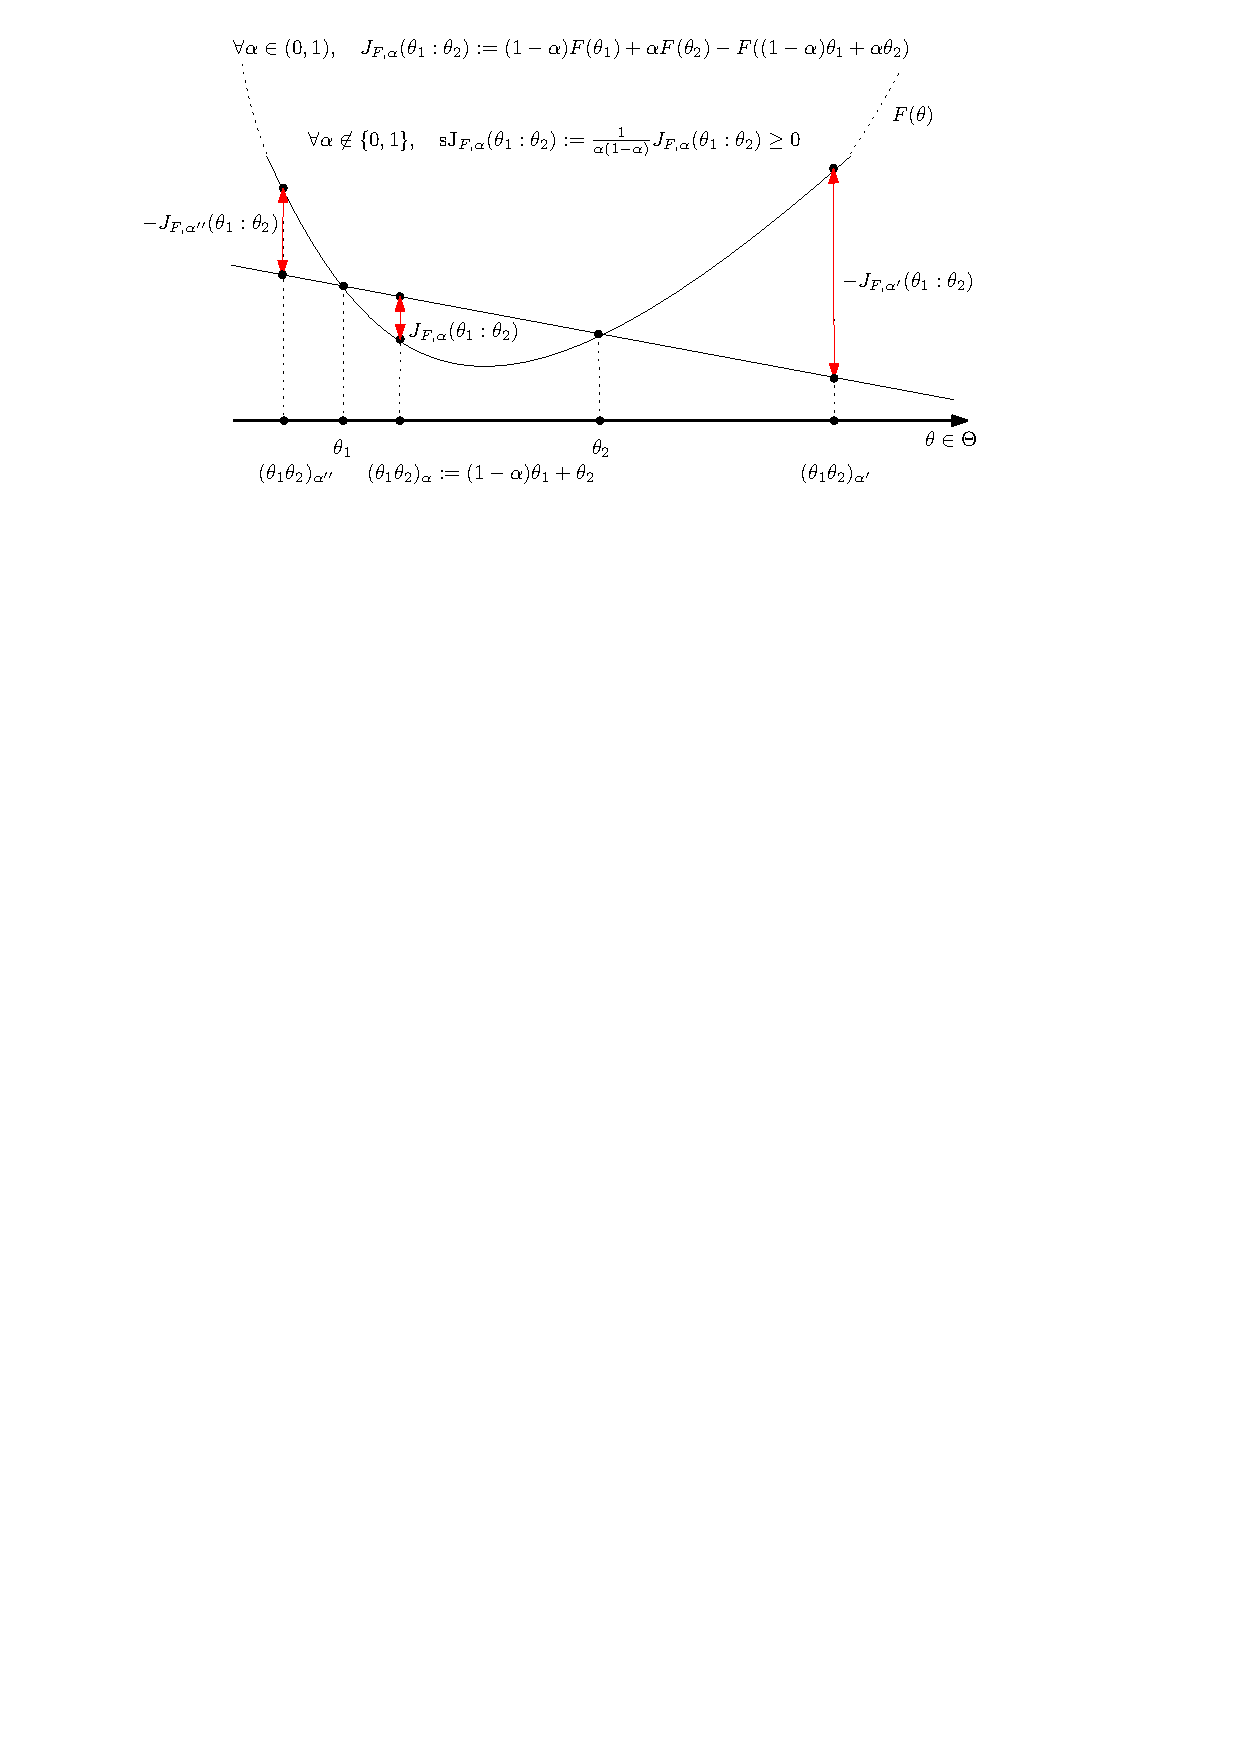
\includegraphics[width=0.75\columnwidth]{FigIpe-skewJS.pdf} 

 
\caption{Skewed Jensen divergences visualized as vertical convexity gaps.}%
\label{fig:JendenDiv}
\end{figure}

%%%
\subsection{Skewed Jensen and Bregman divergences}
%%%

$$
\lim_{\alpha\rightarrow 0} \mathrm{sJ}_{F,\alpha}(\theta_1:\theta_2)=B_F(\theta_1:\theta_2)
$$

$$
\lim_{\alpha\rightarrow 1} \mathrm{sJ}_{F,\alpha}(\theta_1:\theta_2)=B_F(\theta_2:\theta_1)
$$



If $\alpha<0$ or $\alpha>1$, we can measure the gap $F((1-\alpha)\theta_1+\alpha\theta_2)-((1-\alpha) F(\theta_1)+\alpha F(\theta_2))=-J_F(\theta_1,\theta_2)\geq 0$.
See Figure~\ref{fig:JendenDiv}
Thus we can define the scaled $\alpha$-skew Jensen divergence for $\alpha\in\bbR\backslash\{0,1\}$ as:
$$
\sJ_F(\theta_1:\theta_2)=\frac{1}{\alpha(1-\alpha)}J_F(\theta_1:\theta_2)\geq 0.
$$


\subsection{Relationships with statistical distances between densities of an exponential family}

\subsection{Generalizations of Bregman and Jensen divergences}




%%%
\section{Invariant {\protect $f$-divergences}}
%%%%

A $f$-divergence~\cite{Morimoto-1963,EN-PhD-Csiszar-1967,fdiv-AliSilvey-1966,Csiszar-1972} $I_f[p:q]$ is a dissimilarity measure between probability distributions defined for a convex generator $f(u)$:
$$
I_f[p:q]=\int p(x) f\left(\frac{q(x)}{p(x)}\right) \dmu(x).
$$
Using Jensen's inequality, we have $I_f[p:q]\geq f(1)$. Thus we ask for generators satisfying $f(1)=0$.
Moreover, in order to have $I_f[p:q]=0$ iff. $p=q$ ($\mu$-almost everywhere), we require $f(u)$ to be strictly convex at $1$.
The $f$-divergences include many well-known statistical distances listed with their generators: % in Table~\table{tab:fdiv}.

%\begin{table}
\begin{center}
$
\begin{array}{lll}
\text{$f$-divergence } & \text{Formula $I_f[p:q]$} & \text{generator $f(u)$}\\
\hline\hline
\text{Total variation (metric)} & \frac{1}{2}\int |p(x)-q(x)| \dmu(x) & \frac{1}{2} |u-1| \\
\text{Squared Hellinger} & \int (\sqrt{p(x)}-\sqrt{q(x)})^2 \dmu(x) & (\sqrt{u}-1)^2\\
\text{Pearson $\chi^2_P$}  &  \int \frac{(q(x)-p(x))^2}{p(x)} \dmu(x) & (u-1)^2\\
\text{Neyman $\chi^2_N$}  &  \int \frac{(p(x)-q(x))^2}{q(x)} \dmu(x) & \frac{(1-u)^2}{u}\\
\text{Kullback-Leibler} & \int p(x)\log \frac{p(x)}{q(x)} \dmu(x) & -\log u\\
\text{reverse Kullback-Leibler} & \int q(x)\log \frac{q(x)}{p(x)} \dmu(x) & u\log u \\
\text{Jeffreys divergence} &\int (p(x)-q(x))\log\frac{p(x)}{q(x)} \dmu(x) & (u-1)\log u\\
\text{$\alpha$-divergence} &  \frac{4}{1-\alpha^2} (1-\int p^{\frac{1-\alpha}{2}}(x) q^{1+\alpha}(x) \dmu(x))  & \frac{4}{1-\alpha^2}(1-u^{\frac{1+\alpha}{2}})\\ 
\text{Jensen-Shannon} & \frac{1}{2}\int (p(x)\log \frac{2p(x)}{p(x)+q(x)} +  q(x)\log \frac{2q(x)}{p(x)+q(x)})\dmu(x) 
&  -(u+1)\log \frac{1+u}{2} + u\log u\\
\end{array}
$
\end{center}

%\caption{Common $f$-divergences $I_f$ with their corresponding generators. \label{tab:fdiv}}
%\end{table}

 


Two $f$-divergences $I_{f_1}$ and $I_{f_2}$ are equivalent iff. $f_1(u)=f_2(u)+\lambda (u-1)$ for any $\lambda\in\bbR$.
A symmetric $f$-divergence is bounded (e.g., the Jensen-Shannon divergence or the total variation) iff. $f(0)<\infty$. 
The Jeffreys divergence is an unbounded $f$-divergence.
The dual $f$-divergence ${I_f}^*[p:q]:=I_f[p:q]$ is a $f$-divergence for the dual generator $f^*(u)= u f\left(\frac{1}{u}\right)$ (or conjugate generator).
Thus symmetric $f$-divergences (e.g., the Jeffreys divergence, Hellinger divergence, or the Jensen-Shannon divergence) satisfies the functional equality $f(u)=uf(1/u)$.
The $f$-divergences are joint convex and satisfies the information monotonicity property:
$I_f[p_{|\calY}:q_{|\calY}]\leq I_f[p:q]$ for any partition $\calY$ of $\calX$ (see lumping~\cite{TutorialCsiszar-2004}).
A statistical divergence is said separable iff. it can be rewritten as $D[p:q]=\int D_1(p(x):q(x)) \dmu(x)$, where $D_1$ is a scalar divergence. The $f$-divergences are the only divergences which are separable and satisfies the information information monotonicity~\cite{IG-2016} (except the ``curious case''~\cite{fdivBinaryAlphabet-2014} of binary alphabets $\calX$).
A $f$-divergence is said standard~\cite{IG-2016} when $f''(1)=1$. 
The local Taylor expansion~\cite{CharacterizationDiv-1998} of $I_f[p_{\theta_1}:p_{\theta_2}]$-divergences between two parametric divergences is related to the Fisher information matrix $I(\theta)=E_{p_\theta}\left[\nabla \log p_\theta(x) (\nabla \log p_\theta(x))^\top\right]$ as follows:
$$
I_f[p_{\theta_1}:p_{\theta_2}]=\frac{1}{2}(\theta_2-\theta_1)^\top I_\theta(\theta_1)(\theta_2-\theta_1)+o(\|(\theta_2-\theta_1\|^2).
$$ 
Thus we have $I_f[p_{\theta}:p_{\theta+\dtheta}]=\frac{1}{2}\dtheta^\top I(\theta) \dtheta$ for a standard $f$-divergence (with $f''(1)=1$).
The following metric distance $D^\Mah_Q$ is called the Mahalanobis distance~\cite{Mahalanobis-1936}\footnote{Mahalanobis defined that distance for $Q=\Sigma^{-1}\succ 0$, the inverse of a covariance matrix.}:
$$
D^\Mah_Q(\theta_1,\theta_2)=\sqrt{(\theta_2-\theta_1)^\top Q(\theta_2-\theta_1)}.
$$
The  Mahalanobis distance generalizes the Euclidean distance (expressed in the Cartesian coordinate system) using $Q=I$, the identity matrix.
When $\Sigma=\diag(\sigma_{11}^2,\ldots, \sigma_{DD}^2)$ with $\sigma_{ii}=\sigma_i^2$, we have
$$
D^\Mah_{\Sigma^{-1}}(\theta_1,\theta_2)=\sum_{i=1}^D \frac{(\theta_2^i-\theta_1^i)^2}{\sigma_{i}^2}.
$$

Thus we have $I_f[p_{\theta_1}:p_{\theta_2}]=\frac{1}{2}D^\Mah_{I_\theta(\theta_1)}(\theta_1,\theta_2)^2+o(\|(\theta_2-\theta_1\|^2)$.
For $\theta_1=\theta$ and $\theta_2=\theta+\dtheta$, the half squared Mahalanobis distance can be interpreted as the squared Riemannian infinitesimal length element: $I_f[p_{\theta}:p_{\theta+\dtheta}]=\frac{1}{2}\dtheta^\top I_\theta(\theta) \dtheta=\ds_\theta^2$.

A $f$-divergence between any two densities $p_{\theta_1}$ and $p_{\theta_2}$ can be expressed as a Taylor series~\cite{fdivCauchy-2021} when $\frac{p_{\theta_2}(x)}{p_{\theta_1}(x)} < 1+r_f$ 
where $r_f$ is the convergence radius of the analytic generator $f\in C^\omega$ and $\frac{p_{\theta_1}}{p_{\theta_2}}\leq C$:
$$
I_f[p_{\theta_1} : p_{\theta_2}] = \sum_{n=2}^{\infty} a_n \int_{X}  \left( \frac{p_{\theta_2}(x)}{p_{\theta_1}(x)} - 1 \right)^n p_{\theta_1}(x) \dmu(x).
$$
Otherwise, the Taylor series diverge.

By introducing the higher-order chi divergences~\cite{fdivchiorder-2013} 
$$
D_{\chi,n}[p:q]=\int \frac{\left(p(x)-q(x)\right)^n}{(q(x))^{n-1}(x)} \dmu(x)
$$
which are proper divergences for even integers and only pseudo-distances for odd orders, we rewrite the Taylor series of $f$-divergences as:
$$
I_f[p_{\theta_1} : p_{\theta_2}] = \sum_{n=2}^{\infty} a_n D_{\chi,n}[p_{\theta_1} : p_{\theta_2}].
$$

The higher-order chi divergences~\cite{fdivchiorder-2013} between densities of an exponential family are available in closed-form provided that the natural parameter space is affine (e.g., isotropic Gaussian family or Poisson family).

To illustrate the Taylor series, consider the Poisson family, and let us express the Taylor series for the Jensen-Shannon divergence
(generator $f_\JS(u)=-(u+1)\log \frac{1+u}{2} + u\log u$) between two Poisson distributions with parameters $\lambda_1=0.6$ and $\lambda_2=0.3$.
We have the higher-order chi divergences between Poisson distributions expressed in closed-form as follows~\cite{fdivchiorder-2013}:
$$
D_{\chi,k}[p_{\lambda_1}:p_{\lambda_2}]=\sum_{j=0}^k (-1)^{k-j} {k \choose j} e^{\lambda_1^{1-j} \lambda_2^{j} - ((1-j)\lambda_1 +  j\lambda_2)}
$$

Furthermore, $\frac{p_{\lambda_1}(x)}{p_{\lambda_2}(x)}=\frac{\lambda_1^k e^{-\lambda_1}}{\lambda_2^k e^{-\lambda_2}}<C$


We have
$$
I_f[p:q]\sim \frac{f''(1)}{2}D_{\chi^2_N}[p:q],
$$ 
where $D_{\chi^2}[p:q]=\int \frac{(p(x)-q(x))^2}{q(x)} \dmu(x)$ is the chi-squared divergence.
Therefore, we have
\begin{equation}
D_\KL[p:q]\sim \frac{1}{2}D_{\chi^2}[p:q].
\end{equation}


On the finite-dimensional probability simplex, the Kullback-Leibler divergence is the only statistical divergence which belongs to both the $f$-divergences and the Bregman divergences~\cite{AlphaUnique-2009}. When considering the $f$-divergences to positive measures, the intersection of the $f$-divergences and the Bregman divergences are the $\alpha$-divergences~\cite{AlphaUnique-2009}. 

For the parametric family of Cauchy distributions, the $f$-divergences are always symmetric and can be expressed as a function of the chi-squared divergence~\cite{fdivCauchy-2021}:
$$
I_f[p_{l_1,s_1}^\Cauchy:p_{l_2,s_2}^\Cauchy]=I_f[p_{l_2,s_2}^\Cauchy:p_{l_1,s_1}^\Cauchy]=h_f(D_{\chi^2}[p_{l_1,s_1}^\Cauchy:p_{l_2,s_2}^\Cauchy]),
$$
where
$$
D_{\chi^2}[p_{l_1,s_1}^\Cauchy:p_{l_2,s_2}^\Cauchy]=\frac{(l_2-l_1)^2+(s_2-s_1)^2}{2s_1s_2}
$$
and
$$
p_{l,s}^\Cauchy(x) := \frac{1}{\pi s\left(1+\left(\frac{x-l}{s}\right)^2\right)}=\frac{s}{\pi (s^2+(x-l)^2)}.
$$


%%%
\section{Distances and means}
%%%%



%%%
\section{Statistical distances between densities with computationally intractable normalizers}
%%%%

Consider a density $p(x)=\frac{\tilde p(x)}{Z_p}$ where $\tilde p(x)$ is an unnormalized {\em computable} density 
and $Z_p=\int p(x) \dmu(x)$ the {\em computationally intractable} normalizer (also called in statistical physics the partition function or free energy).
A statistical distance $D[p_1:p_2]$ between two densities $p_1(x)=\frac{\tilde p_1(x)}{Z_{p_1}}$ and $p_2(x)=\frac{\tilde p_2(x)}{Z_{p_2}}$ with computationally intractable normalizers $Z_{p_1}$ and $Z_{p_2}$ is said {\em projective} (or two-sided {\em homogeneous}) if and only if
$$
\forall \lambda_1>0,\lambda_2>0,\quad D[p_1:p_2]=D[\lambda_1p_1:\lambda_2 p_2].
$$
In particular, letting $\lambda_1=Z_{p_1}$ and $\lambda_2=Z_{p_2}$, we have
$$
D[p_1:p_2]=D[\tilde{p}_1:\tilde{p}_2].
$$
Notice that the rhs. does not rely on the computationally intractable normalizers.
These projective distances are useful in statistical inference based on minimum distance estimators~\cite{MinDistance-2019} (see next Section).


Here are a few statistical projective distances:

\begin{itemize}
\item {\bf $\gamma$-divergences} ($\gamma>0$)~\cite{gammadivergence-2001,gammadivergence-2008}:
$$
D_{\gamma}[p:q]:=\log \left(\int_{\mathbb{R}} q^{\alpha+1}\right)-\left(1+\frac{1}{\alpha}\right) \log \left(\int_{\mathbb{R}} q^{\alpha} p\right)+\frac{1}{\alpha} \log \left(\int_{\mathbb{R}} p^{\alpha+1}\right),\quad \gamma\geq 0
$$

When $\gamma\rightarrow 0$, we have~\cite{gammadivergence-2008} $D_{\gamma}[p:q]=D_\KL[p:q]$, the Kullback-Leibler divergence (KLD).
For example, we can estimate the KLD between two densities of an exponential-polynomial family by Monte Carlo stochastic integration of the $\gamma$-divergence for a small value of $\gamma$~\cite{PMPEF-2016}.

The $\gamma$-divergences (projective, Bregman-type=Cross-entropy-entropy) and the density power divergence~\cite{BasuPowerDivergence-1998} (non-projective, Bregman-type divergence):
$$
D_{\alpha}^\mathrm{dpd}[p:q]:=\int_{\mathbb{R}} q^{\alpha+1}-\left(1+\frac{1}{\alpha}\right) \int_{\mathbb{R}} q^{\alpha} p+\frac{1}{\alpha} \int_{\mathbb{R}} p^{\alpha+1},\quad \alpha\geq 0,
$$
can be encapsulated into the family of $\Phi$-power divergences~\cite{PhiPowerDivergence-2021} (functional density power divergence class):
$$
D_{\phi, \alpha}[p:q]:=\phi\left(\int_{\mathbb{R}} q^{\alpha+1}\right)-\left(1+\frac{1}{\alpha}\right) \phi\left(\int_{\mathbb{R}} q^{\alpha} p\right)+\frac{1}{\alpha} \phi\left(\int_{\mathbb{R}} p^{\alpha+1}\right),\quad \alpha\geq 0,
$$
where $\phi(e^x)$ convex and strictly increasing, $\phi$ continuous and twice continously differentiable with finite second order derivatives.
We have $D_{\phi,0}[p:q]=\phi'(1)\int_{\mathbb{R}} p(x)\log\frac{p(x)}{q(x)}\dmu(x)=\phi'(1)D_\KL[p:q]$.

\item {\bf Cauchy-Schwarz divergence}~\cite{jenssen2006cauchy} (CSD, projective)
$$
D_\CS[p:q]=-\log \left( \frac{\int p(x) q(x) \dmu(x)}{\sqrt{\int p(x)^{2}  \dmu(x) \int q(x)^{2}  \dmu(x)}} \right) = D_\CS[\lambda_1 p:\lambda_2 q], \forall \lambda_1>0,\lambda_2>0,
$$
and {\bf H\"older divergences}~\cite{HolderDivergence-2017} (HD, projective, which generalizes the CSD):
%$$
%D_{\alpha, \sigma, \tau}^{\mbox{H\"older}}[p:q]=-\log \left(\frac{\int_{\mathcal{X}} p(x)^{\sigma} q(x)^{\tau} \mathrm{d} x}{\left(\int_{\mathcal{X}} p(x)^{\alpha \sigma} \mathrm{d} x\right)^{\frac{1}{\alpha}}\left(\int_{\mathcal{X}} q(x)^{\beta \tau} \mathrm{d} x\right)^{\frac{1}{\beta}}}\right), \quad \frac{1}{\alpha}+\frac{1}{\beta}=1,\alpha\beta>0.
%$$
$$
D_{\alpha, \gamma}^{\mbox{H\"older}}[p:q]=
-\log \left(\frac{\int_{\mathcal{X}} p(x)^{\gamma / \alpha} q(x)^{\gamma / \beta} \mathrm{d} x}{\left(\int_{\mathcal{X}} p(x)^{\gamma} \mathrm{d} x\right)^{1 / \alpha}\left(\int_{\mathcal{X}} q(x)^{\gamma} \mathrm{d} x\right)^{1 / \beta}}\right),\quad \frac{1}{\alpha}+\frac{1}{\beta}=1 .
$$
We have
$$
\forall \lambda_1>0, \lambda_2>0, D_{\alpha, \gamma}^{\mbox{H\"older}}[\lambda_1 p:\lambda_2 q]= D_{\alpha, \gamma}^{\mbox{H\"older}}[p:q],
$$
and
$$
D_{2,2}^{\mbox{H\"older}}[p:q]=D_\CS[p:q].
$$

H\"older divergences between two densities $p_{\theta_p}$ and $p_{\theta_q}$ of an exponential family with cumulant function $F(\theta)$ is available in closed-form~\cite{HolderDivergence-2017}:
$$
D_{\alpha, \gamma}^{\mbox{H\"older}}[p:q]=\frac{1}{\alpha} F\left(\gamma \theta_{p}\right)+\frac{1}{\beta} F\left(\gamma \theta_{q}\right)-F\left(\frac{\gamma}{\alpha} \theta_{p}+\frac{\gamma}{\beta} \theta_{q}\right)
$$

%$$
%D_{\alpha, \sigma, \tau}^{\mbox{H\"older}}[p_{\theta_p}: p_{\theta_q}]=\frac{1}{\alpha} F\left(\alpha \sigma \theta_{p}\right)+\frac{1}{\beta} F\left(\beta \tau \theta_{q}\right)-F\left(\sigma \theta_{p}+\tau \theta_{q}\right).
%$$

The CSD is available in closed-form between mixtures of an exponential family with a conic natural parameter~\cite{nielsen2012closed}: This includes the case of Gaussian mixture models~\cite{kampa2011closed}.
%$$
%D_{\alpha, \sigma, \tau}^{\mathrm{H}}(p: q)=\frac{1}{\alpha} F\left(\alpha \sigma \theta_{p}\right)+\frac{1}{\beta} F\left(\beta \tau \theta_{q}\right)-F\left(\sigma \theta_{p}+\tau \theta_{q}\right).
%$$

\item {\bf Hilbert distance}~\cite{nielsen2019clustering} (projective): Consider two probability mass functions $p=(p_1,\ldots, p_d)$ and $q=(q_1,\ldots,q_d)$ of the $d$-dimensional probability simplex. Then the Hilbert distance is
$$
D^{\mathrm{Hilbert}}[p:q]=\log \left( \frac{\max _{i\in\{1,\ldots, d\}} \frac{p_{i}}{q_{i}}}{\min _{j\in\{1,\ldots, d\}} \frac{p_{j}}{q_{j}}}\right).
$$
We have 
$$
\forall \lambda_1>0, \lambda_2>0, D^{\mbox{Hilbert}}[\lambda_1 p:\lambda_2 q]= D^{\mbox{Hilbert}}[p:q].
$$

The Hilbert projective simplex distance can be extended to the cone of positive-definite matrices~\cite{nielsen2019clustering} (and its subspace of correlation matrices called the elliptope) as follows:
$$
D^{\mathrm{Hilbert}}[P:Q]=\log \left( \frac{\lambda_{\mathrm{max}}(PQ^{-1})}{\lambda_{\mathrm{\min}}(PQ^{-1})} \right),
$$
where $\lambda_{\mathrm{max}}(X)$ and $\lambda_{\mathrm{\min}}(X)$ denote the largest and smallest eigenvalue of matrix $X$, respectively.


\end{itemize}


%%%
\section{Statistical distances between empirical distributions and densities with computationally intractable normalizers}
%%%

When estimating the parameter $\hat\theta$ for a parametric family of distributions $\{p_\theta\}$ from i.i.d. observations $\calS=\{x_1,\ldots,x_n\}$, we can define a minimum distance estimator (MDE):
$$
\hat\theta=\arg\min_\theta D[p_\calS:p_\theta],
$$
where $p_\calS=\frac{1}{n}\sum_{i=1}^n \delta_{x_i}$ is the empirical distribution (normalized).
Thus we need only a right-sided projective divergence to estimate models with computationally intractable normalizers.
For example, the Maximum Likelihood Estimator (MLE) is a MDE wrt. the KLD:
$$
\hat\theta_{\mathrm{MLE}}=\arg\min_\theta D_\KL[p_\calS:p_\theta].
$$
It is thus interesting to study the impact of the choice of the distance $D$ to the properties of the corresponding estimator (e.g., $\gamma$-divergences yields provably robust estimators~\cite{gammadivergence-2008}).



\begin{itemize}
	\item {\bf Hyv\"arinen divergence}~\cite{hyvarinen2005estimation} (also called {\bf Fisher divergence}):
	$$
	D^{\mbox{Hyv\"arinen}}\left[p: p_{\theta}\right]:=\frac{1}{2} \int\left\|\nabla_{x} \log p(x)-\nabla_{x} \log p_{\theta}(x)\right\|^{2}\, p(x) \mathrm{d} x.
	$$
	The Hyvarinen divergence has been extended for order-$\alpha$ Hyvarinen divergences~\cite{nielsen2021fast} (for $\alpha>0$):
	$$
	D^{\mbox{Hyv\"arinen}}_{\alpha}[p: q]:=\frac{1}{2} \int p(x)^{\alpha} \left(\nabla_{x} \log p(x)-\nabla_{x} \log q(x)\right)^{2} \mathrm{d} x, \quad \alpha>0 .
	$$
	
\end{itemize}


\section{The Jensen-Shannon divergence and some generalizations}

%%%
\subsection{Origins of the Jensen-Shannon divergence}
%%%%%

Let $(\calX,\calF,\mu)$ be a measure space, and $(w_1,P_1),\ldots, (w_n,P_n)$ be $n$ weighted probability measures dominated 
by a measure $\mu$ (with $w_i>0$ and $\sum w_i=1$). 
Denote by $\calP:=\{(w_1,p_1),\ldots,  (w_n,p_n)\}$ the set of their weighted Radon-Nikodym densities $p_i=\frac{\mathrm{d}P_i}{\dmu}$ with respect to $\mu$.

A {\em statistical divergence} $D[p:q]$ is a measure of dissimilarity between two densities $p$ and $q$ (i.e., a $2$-point distance) such that $D[p:q]\geq 0$ with equality if and only if $p(x)=q(x)$ $\mu$-almost everywhere.
A {\em statistical diversity index} $D(\calP)$ is a measure of variation of the weighted densities in $\calP$ related to a measure of centrality, i.e., a $n$-point distance which generalizes the notion of $2$-point distance when $\calP_2(p,q):=\{(\frac{1}{2},p_1),(\frac{1}{2},p_2)\}$:
$$
D[p:q]:=D(\calP_2(p,q)).
$$

The fundamental measure of dissimilarity in information theory is the {\em $I$-divergence} (also called the {\em Kullback-Leibler divergence}, KLD,  see Equation~(2.5) page 5~of~\cite{Kullback-1997}):
$$
D_\KL[p:q]:=  \int_\calX p(x)\log\left(\frac{p(x)}{q(x)}\right)\dmu(x).
$$

The KLD is asymmetric (hence the delimiter notation ``:'' instead of `,') but can be symmetrized by defining the Jeffreys {\em $J$-divergence} (Jeffreys divergence, denoted by $I_2$ in Equation (1) in 1946's paper~\cite{Jeffreys-1946}):
$$
D_J[p,q] := D_\KL[p:q]+D_\KL[q:p] = \int_\calX (p(x)-q(x))\log\left(\frac{p(x)}{q(x)}\right)\dmu(x).
$$
Although symmetric, any positive power of Jeffreys divergence fails to satisfy the triangle inequality: 
That is, $D_J^\alpha$ is never a metric distance for any $\alpha>0$, and furthermore $D_J^\alpha$  cannot be upper bounded.

In 1991, Lin proposed the asymmetric {\em $K$-divergence} (Equation (3.2) in~\cite{JS-1991}):
$$
D_K[p:q]:=D_\KL\left[p:\frac{p+q}{2}\right],
$$
and defined the {\em $L$-divergence} by analogy to Jeffreys's symmetrization of the KLD (Equation (3.4) in~\cite{JS-1991}):
$$
D_L[p,q]=D_K[p:q]+D_K[q:p].
$$

By noticing that 
$$
D_L[p,q]= 2 h\left[\frac{p+q}{2}\right]-(h[p]+h[q]),
$$ 
where $h$ denotes Shannon entropy (Equation (3.14) in~\cite{JS-1991}), Lin coined the (skewed) {\em Jensen-Shannon divergence} between two weighted densities $(1-\alpha,p)$ and $(\alpha,q)$ for $\alpha\in(0,1)$ as follows (Equation (4.1) in~\cite{JS-1991}):
\begin{equation}\label{eq:JSh}
D_{\JS,\alpha}[p,q]=h[(1-\alpha)p+\alpha q]-(1-\alpha)h[p]-\alpha h[q].
\end{equation}

Finally, Lin defined the {\em generalized Jensen-Shannon divergence} (Equation (5.1) in~\cite{JS-1991}) for a finite weighted set of densities:
$$
D_\JS[\calP]=h\left[\sum_i w_ip_i\right]-\sum_i w_i h[p_i].
$$
This generalized Jensen-Shannon divergence is nowadays called the {\em Jensen-Shannon diversity index}.

To contrast with the Jeffreys' divergence, the Jensen-Shannon divergence (JSD) $D_\JS:=D_{\JS,\frac{1}{2}}$ is upper bounded by $\log 2$ (does not require the densities to have the same support), and $\sqrt{D_\JS}$ is 
a metric distance~\cite{JSmetric-2003,JSmetric-2004}.
Lin cited precursor work~\cite{WongYOU-1985,JW-1988} yielding definition of the Jensen-Shannon divergence:
The Jensen-Shannon divergence  of Eq.~\ref{eq:JSh} is the so-called ``increments of entropy'' defined in (19) and (20) of~\cite{WongYOU-1985}.

The Jensen-Shannon diversity index was also obtained very differently by Sibson in 1969 when he defined the {\em information radius}~\cite{Sibson-1969} of order $\alpha$ using R\'enyi $\alpha$-means and R\'enyi $\alpha$-entropies~\cite{Renyi-1961}.
In particular, the information radius $\IR_1$ of order $1$ of a weighted set $\calP$ of densities is a diversity index obtained by solving the following variational optimization problem:
\begin{equation}
\IR_{1}[\calP]:=\min_{c} \sum_{i=1}^n w_i D_\KL[p_i:c].  \label{eq:Sibson}
\end{equation}

Sibson solved a more general optimization problem, and obtained the following expression (term $K_1$ in Corollary 2.3~\cite{Sibson-1969}):
$$
\IR_{1}[\calP]=  h\left[\sum_i w_ip_i\right]-\sum_i w_i h[p_i]:=D_\JS[\calP].
$$
Thus Eq.~\ref{eq:Sibson} is a variational definition of the Jensen-Shannon divergence.

%%%
\subsection{Some extensions of the Jensen-Shannon divergence}
%%%%

\begin{itemize}

	\item {\bf Skewing the JSD.} 
	
	The $K$-divergence of Lin can be skewed with a scalar parameter $\alpha\in(0,1)$ to give
	\begin{equation}\label{eq:divK}
	D_{K,\alpha}[p:q]:=D_\KL\left[p:(1-\alpha)p+\alpha q\right].
	\end{equation}
	Skewing parameter $\alpha$ was first studied in~\cite{skewJS-2001} (2001, see Table~2 of~\cite{skewJS-2001}).
	We proposed to unify the Jeffreys divergence with the Jensen-Shannon divergence as follows (Equation 19 in~\cite{nielsen2010family}):
	\begin{equation}\label{eq:JJSalpha}
	D_{K,\alpha}^J[p:q]:=\frac{D_{K,\alpha}[p:q]+D_{K,\alpha}[q:p]}{2}.
	\end{equation}
	When $\alpha=\frac{1}{2}$, we have $D_{K,\frac{1}{2}}^J=D_\JS$, and when $\alpha=1$, we get $D_{K,1}^J=\frac{1}{2}D_J$.
	
	Notice that 
	$$
	D_\JS^{\alpha,\beta}[p;q]:=(1-\beta)D_\KL[p:(1-\alpha)p+\alpha q]+\beta D_\KL[q:(1-\alpha)p+\alpha q]
	$$ 
	amounts to calculate
	 $$
	h^\times[(1-\beta)p+\beta q:(1-\alpha)p+\alpha q]-((1-\beta)h[p]+\beta h[q])
	$$ 
	where 
	$$
	h^\times[p,q]:=\int -p(x)\log q(x)\dmu(x)
	$$ 
	denotes the {\em cross-entropy}. By choosing $\alpha=\beta$, we have $h^\times[(1-\beta)p+\beta q:(1-\alpha)p+\alpha q]=h[(1-\alpha)p+\alpha q]$, 
	and thus recover the skewed Jensen-Shannon divergence of Eq.~\ref{eq:JSh}.
	
	
	In~\cite{nielsen2020generalization} (2020), we considered a positive {\em skewing vector} $\alpha\in [0,1]^k$  and a unit positive weight $w$ belonging to the standard simplex $\Delta_k$, and defined the following {\em vector-skewed Jensen-Shannon divergence}:
\begin{eqnarray}
	D_\JS^{\alpha,w}[p:q] &:=& \sum_{i=1}^k D_\KL[(1-\alpha_i)p_+\alpha_i q : (1-\bar\alpha)p+\bar\alpha q],\\
	&=& h[(1-\bar\alpha)p+\bar\alpha q]-\sum_{i=1}^k h[(1-\alpha_i)p_+\alpha_i q],
\end{eqnarray}
	where $\bar\alpha=\sum_{i=1}^k w_i\alpha_i$. 
	The divergence $D_\JS^{\alpha,w}$ generalizes the (scalar) skew Jensen-Shannon divergence when $k=1$, and is a Ali-Silvey-Csisz\'ar $f$-divergence upper bounded by $\log \frac{1}{\bar\alpha(1-\bar\alpha)}$~\cite{nielsen2020generalization}.
	
	
	\item {\bf A priori mid-density}. The JSD can be interpreted as the total divergence of the densities to the {\em mid-density} $\bar{p}=\sum_{i=1}^n w_i p_i$, a statistical mixture:
	$$
	D_\JS[\calP] = \sum_{i=1}^n w_i D_\KL[p_i:\bar{p}] = h[\bar{p}]-\sum_{i=1}^n w_i h[p_i].
	$$
	Unfortunately, the JSD between two Gaussian densities is not known in closed form because of the definite integral of a log-sum term (i.e., $K$-divergence between a density and a mixture density $\bar{p}$).
	For the special case of the Cauchy family,  a closed-form formula~\cite{CauchyJSD-2021} for the JSD between two Cauchy densities was obtained.
Thus we may choose a {\em geometric mixture distribution}~\cite{JSsym-2019} instead of the ordinary arithmetic mixture $\bar{p}$. More generally, we can choose any weighted mean $M_\alpha$ (say, the geometric mean, or the harmonic mean, or any other power mean) and define a generalization of the $K$-divergence of Equation~\ref{eq:divK}:
	\begin{equation}
	D_K^{M_\alpha}[p:q] := D_K[p:(pq)_{M_\alpha}],
	\end{equation}
	where 
	$$
	(pq)_{M_\alpha}(x):=\frac{M_\alpha(p(x),q(x))}{Z_{M_\alpha}(p:q)}
	$$
	 is a statistical $M$-mixture with $Z_{M_\alpha}(p,q)$
	denoting the normalizing coefficient:
	$$
	Z_{M_\alpha}(p:q)=\int M_\alpha(p(x),q(x))\dmu(x)
	$$ 
	so that $\int (pq)_{M_\alpha}(x)\dmu(x)=1$.
	These $M$-mixtures are well-defined provided the convergence of the definite integrals.
	
	Then we define a generalization of the JSD~\cite{JSsym-2019} termed {\em $(M_\alpha,N_\beta)$-Jensen-Shannon divergence} as follows:
		\begin{equation}
	D_\JS^{M_\alpha,N_\beta}[p:q ]:= N_\beta\left(D_K[p:(pq)_{M_\alpha}] , D_K[q:(pq)_{M_\alpha}]\right),
	\end{equation}
	where $N_\beta$ is yet another weighted mean to average the two $M_\alpha$-$K$-divergences. 
	We have $D_\JS=D_\JS^{A,A}$ where $A(a,b)=\frac{a+b}{2}$ is the arithmetic mean.
	The geometric JSD yields a closed-form formula between two multivariate Gaussians, and has been used in deep learning~\cite{VIGJSD-2020}.
		More generally, we may consider the Jensen-Shannon symmetrization of an arbitrary distance $D$ as  
			\begin{equation}
	D^\JS_{M_\alpha,N_\beta}[p:q]:= N_\beta\left(D[p:(pq)_{M_\alpha}],D[q:(pq)_{M_\alpha}]\right).
	\end{equation}
 %We have the JS-symmetrization of the reverse KLD with respect to the geometric mean which amounts to the skewed Bhattacharyya divergence: $(D_\KL^*)_{G_\alpha}^\JS=D_{\mathrm{Bhat},1-\alpha}$.
	
	\item {\bf A posteriori mid-density}.
	We consider a generalization of Sibson's information radius~\cite{Sibson-1969}.
	Let $S_w(a_1,\ldots,a_n)$ denote a generic weighted mean of $n$ positive scalars $a_1,\ldots, a_n$, with weight vector $w\in\Delta_n$.
	Then we define the {\em $S$-variational Jensen-Shannon diversity index}~\cite{vJSD-2021} as
	\begin{equation}
	D_\vJS^{S_w}(\calP) := \min_{c} S_w\left(D_\KL[p_1:c],D_\KL[p_n:c]\right).
	\end{equation}
	When $S_w=A_w$ (with $A_w(a_1,\ldots,a_n)=\sum_{i=1}^n w_i a_i$ the arithmetic weighted mean), we recover the ordinary Jensen-Shannon diversity index.
			More generally, we define the {\em $S$-Jensen-Shannon index of an arbitrary distance $D$} as
	\begin{equation}
D^\vJS_{S_w}(\calP):=\min_{c} S_w\left(D[p_1:c],\ldots, D[p_n:c]\right).	
\end{equation}
When $n=2$, this yields a Jensen-Shannon-symmetrization of distance $D$.

The variational optimization defining the JSD can also be constrained to a (parametric) family of densities $\calD$, thus defining 
	the {\em $(S,\calD)$-relative Jensen-Shannon diversity index}:
	\begin{equation}
	D_\vJS^{S_w,\calD}(\calP) := \min_{c\in\calD} S_w\left(D_\KL[p_1:c],\ldots, D_\KL[p_n:c]\right).
	\end{equation}
	

The relative Jensen-Shannon divergences are useful for clustering applications:
Let $p_{\theta_1}$ and $p_{\theta_2}$ be two densities of an exponential family $\mathcal{E}$ with cumulant function $F(\theta)$.
Then the $\mathcal{E}$-relative Jensen-Shannon divergence is the Bregman information of $\calP_2(p,q)$ for the conjugate function $F^*(\eta)=-h[p_\theta]$ 
(with $\eta=\nabla F(\theta)$). The $\calE$-relative JSD amounts to  a {\em Jensen divergence} for $F^*$:

\begin{eqnarray}
D_\vJS[p_{\theta_1},p_{\theta_2}] &=& \min_\theta \frac{1}{2}\left\{D_\KL[p_{\theta_1}:p_{\theta}]+D_\KL[p_{\theta_2}:p_{\theta}]\right\},\\
 &=& \min_\theta \frac{1}{2}\left\{B_F[\theta:\theta_1]+B_F[\theta:\theta_2]\right\},\\
 &=&  \min_\eta  \frac{1}{2}\left\{B_{F^*}[\eta_1:\eta]+B_{F^*}[\eta_2:\eta]\right\},\\
&=& \frac{F^*(\eta_1)+F^*(\eta_2)}{2}-F^*(\eta^*),\\
&=:& J_{F^*}(\eta_1,\eta_2),
\end{eqnarray}
since $\eta^*:=\frac{\eta_1+\eta_2}{2}$ (a right-sided {\em Bregman centroid}~\cite{SBD-2009}).
 

	



\end{itemize}

%%%
\section{Statistical distances between mixtures}
%%%%

Pearson~\cite{pearson1894contributions} first considered a unimodal Gaussian mixture of two components for modeling distributions crabs in 1894.
Statistical mixtures~\cite{mclachlan1988mixture} like the Gaussian mixture models (GMMs) are often met in information sciences, and therefore it is important to assess their dissimilarities.
Let $m(x)=\sum_{i=1}^k w_i p_i(x)$ and  $m'(x)=\sum_{i=1}^{k'} w_i' p_i'(x)$ be two finite statistical mixtures.
The KLD between two GMMs $m$ and $m'$ is not analytic~\cite{KLnotanalytic-2004} because of the log-sum terms:
$$
D_\KL[m:m']=\int m(x)\log\frac{m(x)}{m'(x)} \dx.
$$
However, the KLD between two GMMs with the same prescribed components $p_i(x)=p_i'(x)=p_{\mu_i,\Sigma_i}(x)$ (i.e., $k=k'$, and only the normalized positive weights may differ) is provably a Bregman divergence~\cite{wmixtures-2018} for the differential negentropy $F(\theta)$: 
$$
D_\KL[m(\theta):m(\theta')]=B_F(\theta,\theta'),
$$
where $m(\theta)=\sum_{i=1}^{k-1} w_ip_i(x)+(1-\sum_{i=1}^{k-1} w_i)p_k(x)$ and
$F(\theta)=\int m(\theta)\log m(\theta)\dx$. The family $\{m_\theta\: \ \theta\in\Delta_{k-1}^\circ\}$ is called a mixture family in information geometry, where $\Delta_{k-1}^\circ$ denotes the $(k-1)$-dimensional open standard simplex.
However, $F(\theta)$ is usually not available in closed-form because of the log-sum integral.
In some special cases like the mixture of two prescribed Cauchy distributions, we get a closed-form formula for the KLD, JSD, etc.~\cite{CauchyJSD-2021,nielsen2021dually}.
Thus when dealing with mixtures (like GMMs), we either need efficient approximating  (\S\ref{sec:mix:approx}), bounding (\S\ref{sec:mix:bound}) KLD techniques, or new distances (\S\ref{sec:mix:newdist}) that yields closed-form formula between mixture densities.

% , or estimating (\S\ref{sec:mix:est})


%%
\subsection{Approximating and/or fast statistical distances between mixtures}\label{sec:mix:approx}
%%

\begin{itemize}
	\item The Jeffreys divergence (JD) $D_J[m,m']=D_\KL[m:m']+D_\KL[m':m]$ between two (Gaussian) MMs is not available in closed-form, and can be estimated using Monte Carlo integration as 
	$$
\hat{D}_J^{\calS_s}[m,m'] :=   \frac{1}{s} \sum_{i=1}^s 2\frac{(m(x_i)-m'(x_i))}{m(x_i)+m'(x_i)}\log\left(\frac{m(x_i)}{m'(x_i)}\right),
$$
where $\calS_s=\{x_1,\ldots, x_s\}$ are $s$ IID samples from the mid mixture $m_{12}(x):=\frac{1}{2}(m(x)+m'(x))$ (with $\lim_{s\rightarrow \infty} \hat{D}_J^{\calS_s}[m,m']=D_J[m,m']$).
 In~\cite{JeffreysGMMPEF-2021}, the mixtures $m$ and $m'$ are converted into densities of an exponential-polynomial family.
The JD between densities $p_\theta$ and $p_{\theta'}$ of an exponential family with cumulant function $F$ is available in closed-form:
$$
D_J[p_\theta,p_{\theta'}]=(\theta'-\theta)\cdot (\eta'-\eta),
$$ 
with $\eta=\nabla F(\theta)$ and $\theta=\nabla F^*(\eta)$, where $F^*$ denotes the convex conjugate.
Any smooth density $r$ (includes a mixture $r=m$) is converted into  close densities $p_{\theta_r^\MLE}$ and $p^{\eta_r^\SME}$ of a exponential-polynomial family using
extensions of the Maximum Likelihood Estimator (MLE) and Score Matching Estimator (SME).
Then JD between mixtures is approximated as follows
$$
D_J[m,m']\simeq ({\theta'}^\SME-\theta^\SME)\cdot ({\eta'}^\MLE-\eta^\MLE).
$$

\item Given a finite set of mixtures $\{m_i(x)\}$ sharing the same components (e.g., points on a mixture family manifold), we precompute the KLD between  pairwise components to obtain fast approximation of the KLD $D_\KL[m_i:m_j]$ between any two mixtures $m_i$ and $m_j$, see~\cite{Comix-2016}.
 
\end{itemize}





%%
\subsection{Bounding statistical distances between mixtures}\label{sec:mix:bound}
%%

\begin{itemize}

\item {\bf Log-Sum-Exp bounds}: In~\cite{LSE-MM1D-2016,alphadiv-2017}, we lower and upper bound the cross-entropy between mixtures using the fact that the log-sum term $\log m(x)$ and be interpreted as a LSE function. We then compute lower envelopes and upper envelopes of density functions using technique of computational geometry to report deterministic lower and upper bounds on the KLD and $\alpha$-divergences. These bounds are said combinatorial because we decompose the support into elementary intervals. Bounds between the Total Variation Distance (TVD) between univariate mixtures are reported in~\cite{TVmixture-2018}.



\end{itemize}



%\subsection{Estimating statistical distances between mixtures}\label{sec:mix:est}


\subsection{Newly designed statistical distances yielding closed-form formula for mixtures}\label{sec:mix:newdist}


\begin{itemize}
	\item {\bf Statistical Minkowski distances}~\cite{StatMinkGMM-2019}:
	Consider the   Lebesgue space 
	$$
	L_\alpha(\mu)  \eqdef \left\{ f\in \bbF \st  \int_\calX |f(x)|^\alpha \dmu(x) <\infty \right\}
	$$  
	for $\alpha\geq 1$, where   $\bbF$ denotes the set of all real-valued measurable functions defined on the support $\calX$. Minkowski's inequality writes as
$\|p+q\|_\alpha \leq \|p\|_\alpha+\|q\|_\alpha$ for $\alpha\in [1,\infty)$.
 The statistical Minkowski difference distance between $p,q\in L_\alpha(\mu)$ is defined as
\begin{equation}
D_\alpha^{\mathrm{Minkowski}}[p,q] \eqdef \|p\|_\alpha+\|q\|_\alpha - \|p+q\|_\alpha\geq 0.
\end{equation}
The statistical Minkowski log-ratio distance is defined by:
\begin{equation}
L_\alpha^{\mathrm{Minkowski}}[p,q] \eqdef -\log \frac{\|p+q\|_\alpha}{\|p\|_\alpha+\|q\|_\alpha}\geq 0.
\end{equation}
These statistical Minkowski distances are symmetric, and $L_\alpha[p,q]$ is scale-invariant.
For even integers $\alpha\geq 2$, $D_\alpha^{\mathrm{Minkowski}}[m:m']$ is available in closed-form.


\item We show that the Cauchy-Schwarz divergence (CSD), the quadratic Jensen-R\'enyi divergence~\cite{JRGMM-2009} (JRD), and the total square Distance (TSD) between two GMMs, and more generally two mixtures of exponential families, can be obtained in closed-form in~\cite{nielsen2012closed}.
\end{itemize}



%%%
%\section{Distances between exponential family densities}
%%%%
%
%\cite{KLDSigmaPts-2021}
%
%\cite{OnicescuEF-2020}
%
%
%$q$-divergences between $q$-exponential family densities

\vskip 1cm
Initially created 13th August 2021 (last updated \today).

\bibliographystyle{plain}
\bibliography{DistanceBib}
\end{document}
